\documentclass[twocolumn]{ctexart}
\usepackage{ctex}
\usepackage{amsmath}

%首行缩进两字符 利用\indent \noindent进行控制
\usepackage{indentfirst}
\setlength{\parindent}{2em}

%算法包
\usepackage{caption}
\usepackage{algorithm}
\usepackage{algorithmic}

%页边距包
\usepackage{geometry}
\geometry {left=2.0cm ,right=2.0cm,top=2.5cm,bottom=2.5cm}

%枚举
\usepackage{enumerate}

%算法input output
\renewcommand{\algorithmicrequire}{\textbf{Input:}} % Use Input in the format of Algorithm
\renewcommand{\algorithmicensure}{\textbf{Output:}} % Use Output in the format of Algorithm

%数学符号
\usepackage{amssymb}
\usepackage{wasysym}
%图片
\usepackage{graphicx}

%表格
\usepackage{booktabs}
\usepackage{multirow}

%Tikz画图
\usepackage{tikz}
\usetikzlibrary{arrows,graphs} %指明是图库
%\usegdlibrary
\begin {document}
	\title{Problem Set 4 Answer Sheet}
	\author{\textbf{151220131谢旻晖}}
	\date{}
	\maketitle
	
\section*{Problem 5.1}
\begin{algorithm}
	\caption{NON\_RECURSIVE\_DFS}
	\label{NON_RECURSIVE}
	\begin{algorithmic}[1]
		\STATE \textbf{procedure} DFSSweep(G)
		\STATE //初始化颜色为white
		\FOR{each vertex \textbf{v} in V}
			\STATE color[v]=white
		\ENDFOR
		\FOR{each vertex \textbf{v} in V}
		\IF{color[v]==white}
			\STATE dfs(v)
		\ENDIF
		\ENDFOR
		\STATE \textbf{end procedure}
		\STATE  
		\STATE  //子过程dfs
		\STATE \textbf{procedure} dfs(v)
			\STATE color[v] = gray
			\STATE stack.push(v)
			\WHILE {!stack.empty}
				\STATE	v=stack.top()
				\STATE v\_isfinished=true
				\FOR {each \textbf{u} in adj[v]}
					\IF{color[u]==white}
						\STATE color[u]=grey
						\STATE push(u)
						\STATE v\_isfinished=false
						\STATE \textbf{break}
					\ENDIF
					
					\IF{v\_isfinished}
						\STATE color[v]=black
						\STATE stack.pop() //把v出栈
					\ENDIF
				\ENDFOR
			\ENDWHILE
		\STATE \textbf{end procedure}		
	\end{algorithmic}
\end{algorithm}
\indent 算法见\textbf{Algorithm }\ref{NON_RECURSIVE}

\section*{Problem 5.2}
\indent 只可能是CE。
\indent 说明如下:在u发现之前v已经完成了遍历,也即点着色为u白色,v黑色,显然只可能是Cross Edge

\section*{Problem 5.3}
\indent 采用反证法证明,如果一个收缩图有从强连通片x到强连通片y的环,即有强连通片x到强连通片y的有向路径$x \leadsto y$,同时也有强连通片y到强连通片x的有向路径$y \leadsto x$,那么x与y就相互可达,这与x,y都是强连通片矛盾。


\section*{Problem 5.4}
\indent 第一次DFS不可以被替换为BFS,原因是:第一次DFS中每遍历完成一个点有一个post order的入栈操作,这是BFS不可完成的。\\

\indent 而第二次DFS仅仅是为了遍历而已,可以被替换为BFS。

\section*{Problem 5.5}
\noindent DFS树根v是割点的充要条件为:v有两棵及两棵以上子树。\\
\noindent 证明:\\
\indent $\Longrightarrow$:\\
\indent 采用反证法,如果结论不成立,那么v没有或有1棵子树。如果v没有子树,则图为平凡图或不连通图,显然v不是割点,矛盾;如果v只有一个子树,则去掉v之后剩下的图也显然连通,矛盾;所以v有两棵及两棵以上子树。\\
\indent $\Longleftarrow$: \\
\indent 显然成立,去掉v之后两棵子树不再连通了。

\section*{Problem 5.6}
\indent 仍然可以正确。$back(v)$的意义为v的所有子树的back edge能回溯到的最早的$discovertime$,当v可以回溯到更早的结点时,$back(v)$就一定会被更新了。如果v不是割点,那么经过更新缩小后的$back(v)$一定小于等于$discovertime(v.parent)$。所以把$back(v)$初值往大里放缩,我们只是先初始化所有点为割点而已,再一个个筛去非割点的点而已,并没有影响。\\


\section*{Problem 5.7}
\noindent 1.\\
\indent 首先证明引理:若无向图G中各顶点的度均大于或等于2,则G中必有回路。证明:在图G中寻找一条最长路P, 并设其最后一个节点为v, 考察v的邻点.易知, v的所有邻点都在P上, 否则, 若u是v的一个不在P上的邻点, 则$P+v\rightarrow u$是一条更长的路, 矛盾.由于G中每个顶点的度都大于等于2, 故v存在一个邻点x, 且x在P上, 但x与v在P上不相邻, 此时路$x\xrightarrow{P}v$与$v\rightarrow x$就构成了一个环.\\
\indent 接着证明原命题:如果图中有度为1的点,那么删除任意一个这样的点之后G显然仍然连通;如果图中没有度为1的点,那么图中所有点的度数均$\ge2$,由引理图必定存在环,删除环上的任意一点之后,G仍然连通。\\
\noindent2.\\
%\begin{tikzpicture}[>=stealth, every node/.style={circle, draw, minimum size=0.75cm}]
%\graph
%{
%	1 -> 2;
%	2 -> 3;
%	3 -> 1;
%};  
%\end{tikzpicture}
\begin{center}
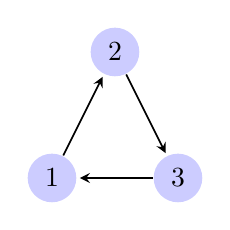
\begin{tikzpicture}
[> = stealth, % arrow head style
shorten > = 1pt, % don't touch arrow head to node
auto,
node distance = 3cm, % distance between nodes
semithick % line style
,scale=.8,auto=left,every node/.style={circle,fill=blue!20}]
\node (n1) at (0,0) {1};
\node (n2) at (1,2)  {2};
\node (n3) at (2,0)  {3};
\draw[->] (n1)->(n2);
\draw[->] (n2)->(n3);
\draw[->] (n3)->(n1);
\end{tikzpicture}
\end{center}

\noindent 3.\\
\begin{center}
	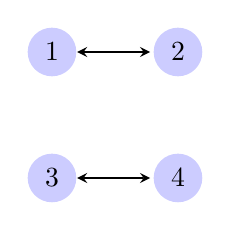
\begin{tikzpicture}[> = stealth, % arrow head style
	shorten > = 1pt, % don't touch arrow head to node
	auto,
	node distance = 3cm, % distance between nodes
	semithick % line style
	,scale=.8,auto=left,every node/.style={circle,fill=blue!20}]
	\node (n1) at (0,0) {1};
	\node (n2) at (2,0)  {2};
	\node (n3) at (0,-2)  {3};
	\node (n4) at (2,-2)  {4};
	\draw[<->] (n1)->(n2);
	\draw[<->] (n3)->(n4);
	\end{tikzpicture}
\end{center}




\section*{Problem 5.8}
\indent 该算法仅仅检测了由一条BE $v\rightarrow w$和一些TE形成的路径$w\leadsto v$构成的环,而对于由两条BE,一些TE构成的环无法检测。例子如下:下图中用红色加粗标记的环长为3的最小环$1\rightarrow 4\rightarrow5\rightarrow1$无法被检测到,这就导致了算法的错误。
\begin{center}
	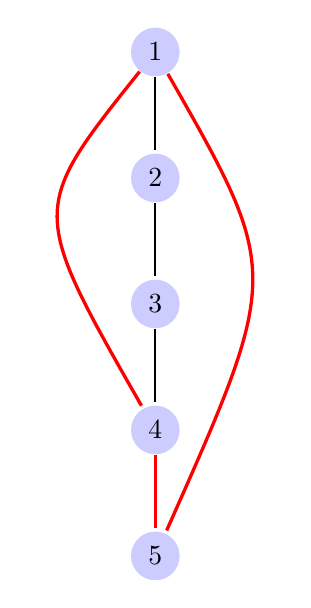
\begin{tikzpicture}[> = stealth, % arrow head style
	shorten > = 1pt, % don't touch arrow head to node
	auto,
	node distance = 3cm, % distance between nodes
	semithick % line style
	,scale=.8,auto=left,every node/.style={circle,fill=blue!20}]
	\node (n1) at (0,0)		{1};
	\node (n2) at (0,-2)  	{2};
	\node (n3) at (0,-4) 	{3};
	\node (n4) at (0,-6) 	{4};
	\node (n5) at (0,-8) 	{5};
	\draw (n1)--(n2);
	\draw (n2)--(n3);
	\draw (n3)--(n4);
	\draw [red,very thick](n4)--(n5);
	\draw [red,very thick] (n1) .. controls (-2,-2.5)  ..(n4);
	\draw [red,very thick](n1) .. controls (2,-3.5) 	..(n5);
	\end{tikzpicture}
\end{center}


\section*{Problem 5.10}
\indent 首先易证如果这个图有2个及以上的入度为0的点,这个DAG就不存在哈密顿通路。基于这个事实,对原来的DAG进行一次拓扑排序,在拓扑排序途中如果有2个及以上入度为0的点,就不存在哈密顿通路。拓扑排序顺利结束,则存在这样一条哈密顿通路,且拓扑序就是通路点序列。

\section*{Problem 5.11}


\begin{algorithm}
	\caption{TOPO\_SORT}
	\label{TOPO_SORT}
	\begin{algorithmic}[1]
	\STATE 	degree[1...$\lvert V \rvert$] //所有结点的入度数组
	\STATE queue
	\STATE  统计所有点的入度,存入degree[]
	\STATE queue.push(所有入度为0的点)
	\WHILE{\NOT queue.empty()}
		\STATE v=queue.pop() //取出队头元素
		\FOR {\textbf{each} j in adj(v)}
			\STATE degree[j]=degree[j]-1
			\IF{degree[j]==0}
				\STATE queue.push(j)
			\ENDIF
		\ENDFOR
	\ENDWHILE
	

	\end{algorithmic}
\end{algorithm}
\noindent1.\\
\indent 算法思想:维护一个入度为0的点队列:初始化时统计所有点的入度,将入度为0的点进队。只要队列不为空,就取出队头并输出,同时处理以队头为起点的所有有向边,将边的终点的入度减一,如果减到0了,就入队。\\
\indent 算法伪代码,见\textbf{Algorithm }\ref{TOPO_SORT}\\
\indent 算法复杂度:一个点最多入队一次,一条边最多被删去一次,所以整体复杂度为$O(m+n)$\\

\noindent2.\\
\indent 会在算法执行到一定时候找不到入度为0的点,非正常退出,拓扑排序无法完成。\\

\section*{Problem 5.12}
\noindent 1.\\
\indent DFS(s),看是否可以遍历完所有点。\\

\noindent2.\\
\indent 使用SCC收缩有向图G,设收缩之后的DAG图为G'。对G'进行拓扑排序,对起点(排序为第一的)进行一次DFS,如果可以遍历完G'中的所有点,则存在这样一个"one-to-all"的顶点,否则不存在。\\
\indent 整体复杂度=SCC+拓扑排序+一次DFS=$O(m+n)$


\section*{Problem 5.13}
首先,可以很容易证明同一连通分量中的点的影响力值是相同的。\\
\noindent 1.\\
\indent \textbf{STEP 1:}对原图G,进行SCC收缩,形成分量收缩图G'。\\
\indent \textbf{STEP 2:}找到出度为0的那些连通分量收缩点,其中包含最少点数的那个连通分量中所有的点是影响力最小的点。\\
\indent 整体复杂度$=O(m+n)+O(n)+O(n)=O(m+n)$。\\
\noindent 2.\\
\indent \textbf{STEP 1:}对原图G,进行SCC收缩,形成分量收缩图G'。\\
\indent
\textbf{STEP 2:}找到入度为0的那些连通分量收缩点,对其中的每个连通分量收缩点的某一点$x$进行一次DFS,同时记录下这个$x$可达的顶点个数,也即是该$x$所属的连通分量中任意一点的影响力。\\
\indent \textbf{ STEP 3:}找出其中影响力最大的连通分量,该分量中任意一点都是影响力最大的点。\\
\indent 整体复杂度$=O(m+n)+n*O(m+n)+O(n)=O(mn+n^2)$\\

\section*{Problem 5.14}
\indent 对原图求关键路径,关键路径长度即为最少学期数。\\
\indent 算法复杂度为$O(m+n)$。\\



\section*{Problem 5.16}
\noindent 1.\\
\indent 将问题建成图模型,每个小孩子都是一个顶点,如果"i恨j",则向图中添加一条$i\rightarrow j$的有向边,最终形成的图为G。\\
\indent
进行一次DFS检测是否有环,若无环,根据结点的$finishTime$对G进行逆拓扑排序,逆拓扑排序的顺序就是小孩排队的顺序;否则,G存在环,不存在符合条件的排队方法。\\

\noindent 2.\\
\indent 将问题建成图模型,每个小孩子都是一个顶点,如果"i恨j",则向图中添加一条$i\rightarrow j$的有向边,最终形成的图为G。\\
\indent
利用DFS求出G的关键路径长度,即为最少行数。若G有环(即DFS中有$Back\ Edge$),此时不存在满足要求的排法。\\

\section*{Problem 5.18}
\indent \textbf{BE:}当某个点发现一条BE时,由无向图的特性,祖先早已用这条边遍历了它,这就矛盾了。\\
\indent \textbf{FE:}由于BFS没有回退的过程,所以绝对没有FE。




\section*{Problem 5.19}
\noindent 1.\\
\indent 可以的,我们设图的两部分可以最终被着色为蓝和红色。我们从任意一点开始,把他染成蓝色,进行无向图的DFS。\\
\indent 在DFS的过程中:$preorder$部分,将该结点染成\textbf{非}父结点颜色的颜色;每当即将访问一个已经访问过的点(Check NonTree Edge),检测该点与自身是否颜色不同,如果相同,则该图不是二部图。完成遍历之后,判定该图为二部图。\\
\noindent 2.\\
\indent 本题显然使用BFS更佳,BFS与DFS的优劣对比如下:\\
\indent \textbf{从处理角度来看:}DFS在有$post order$后序的处理时有优势,BFS则没有后序处理。\\
\indent \textbf{从问题类型来看:}DFS对于解决遍历和求所有问题有效,对于问题搜索深度小的时候处理速度迅速,然而在深度很大的情况下效率不高;BFS对于解决最短或最少问题特别有效,而且寻找深度小。\\


\section*{Problem 5.20}
\indent 从任意一点进行DFS,如果遇到了$BackEdge$,那么就可以移除它,且去掉之后G仍然连通(由于DFS生成树),否则就不存在。\\
\indent 算法复杂度分析:无向图的DFS中只存在$TreeEdge$和$BackEdge/ForwardEdge$(从不同方向看类型不同)。且最多有$n-1$条$TreeEdge$边,当检测到第$n$条边的时候他一定是$BackEdge/ForwardEdge$,这就保证了我们的算法最多只要检测$n$条边,所以复杂度为$O(n)$。\\


\section*{Problem 5.22}
%\begin{algorithm}
%	\caption{PERFECT\_SUBTREE($root$)}
%	\label{MAX_PERFECT_SUBTREE}
%	\begin{algorithmic}[1]
%	\REQUIRE root为树的根结点
%%	\ENSURE [h,isPerfect,TREE\_SET] h为树的高度,isPerfect代表是完美二叉树,TREE\_SET完美子树集;其中前两者为过渡%参数,第三个为最终结果。
%		\IF{root==NULL}
%			\RETURN [0,$true$,NULL]
	%	\ENDIF
%		\STATE %[$h_L$,$isPerfect_L$,TREE\_SET\_L]=PERFECT\_SUBTREE($root->left$)
%		\STATE [$h_R$,$isPerfect_R$,TREE\_SET\_R]=PERFECT\_SUBTREE($root->right$)
	%	\IF{$h_L==h_R $ \&\& $isPerfect_L$ \&\& $isPerfect_R$}
%			\RETURN [$h_L+1$,$true$,root]
	%	\ELSE
%			\RETURN[$max(h_L,h_R)+1$,$false$,max(TREE\_SET\_L,TREE\_SET\_R)]
%			\STATE %//返回树高,和完美子树集,此处对两个树集合的max操作返回\textbf{所有}%最大的树的集合
%		\ENDIF
%	\end{algorithmic}
%\end{algorithm}


%\indent 可以写出一个分治的算法:一棵树的最大完美子树是什么,基于他的子树们的状态确定:\\
%如果双子树都是完美二叉树,且高度相同,最大完美子树就是自己;\\
%如果只有一棵子树,最大完美子树就是儿子的最大完美子树;\\
%其他情况,就是左右子树的最大完美子树中最大的那一个或一些(最大的有多棵)。\\
%算法伪代码见\textbf{Algorithm }\ref{MAX_PERFECT_SUBTREE}。

\begin{algorithm}
	\caption{PERFECT\_SUBT($root$)}
	\label{MAX_PERFECT_SUBTREE}
	\begin{algorithmic}[1]
	\REQUIRE root为树的根结点
	\ENSURE [h,isPerfect] h为树的高度,isPerfect是一个布尔型变量代表是完美二叉树
	\STATE \textbf{GLOABL} $queue$
	\IF{root==NULL}
			\RETURN [0,$true$]
	\ENDIF
		\STATE[$h_L$,$isPerfect_L$]=PERFECT\_SUBTREE($root->left$)
		\STATE [$h_R$,$isPerfect_R$]=PERFECT\_SUBTREE($root->right$)
	\IF{$h_L==h_R $ \&\& $isPerfect_L$ \&\& $isPerfect_R$}
			\STATE $queue$.push([$h_L+1$,root])
			\WHILE{$queue$.top().h<$h_L+1$}
				\STATE $queue$.pop()
				\STATE //让队列前端树高小于当前元素的树们出队
			\ENDWHILE
			\RETURN [$h_L+1$,$true$]
	\ELSE
			\RETURN[$max(h_L,h_R)+1$,$false$]
			\STATE //返回树高,false代表非完美二叉树
	\ENDIF
	\end{algorithmic}
\end{algorithm}



\indent 算法思路:维护一个存有当前最大的完美二叉树\textbf{集}的队列$queue$,$queue$中元素具有的形式为[h,root],h为树高,root为树根。每当向队列中压入一棵完美二叉树时,就把队头所有高度小于他的树全部出队。这样,算法结束后,队列中所有树就是最大完美子树。\\
\indent
算法伪代码见\textbf{Algorithm} \ref{MAX_PERFECT_SUBTREE}。\\


\section*{Problem 5.24}
\noindent 1.\\
\indent \textbf{DFS--有向图:}当检测到有$Back Edge$时,原图有环。\\
%\indent \textbf{DFS--无向图:}无向图只有$Tree Edge$和$Back Edge$,所以检测到有$Back Edge$时,原图有环。\\
%\indent \textbf{BFS--有向图:}\\
\indent \textbf{BFS--无向图:}无向图只有$Tree Edge$和$Cross Edge$,所以检测到有$Cross Edge$时,原图有环。\\


\noindent 2.\\
\indent 采用这样的$adversary$策略,对于顶点个数$n$,构造一个$|E|=n^2$条有向边的图,则$O(n)$的算法不可能遍历完所有的边。可以构造这样的一个恶意输入,使得算法老师的算法遍历到的边没有环,而剩下的边我们随意构造出一个环,使得算法产生错误的结果,这就证明了算法老师的算法的错误性。\\

\section*{Problem 5.25}
\noindent 1.\\
\indent 由于边权值为1,任何生成树都是最小生成树。所以,从任意一点出发进行一次DFS,得到生成树,权为$n-1$。\\

\noindent 2.\\
\indent 使用DFS找出所有的非割边,从中删去权值最大的一条,重复11次,直到剩下$m=n-1$条边即为MST。\\
\indent 算法复杂度为$11*O(n+m)=O(n)$。


\noindent 3.\\
\indent
使用类似kruskal算法的方法,首先将所有边分类为权值为1的和为2的;去掉原图中的所有边,往图里不断加入权值小的(权为1的用完了用权为2的)且不构成环的边,直到图所有结点连通。\\
\indent 算法复杂度为:边分类$O(m)$,不断加边要加$O(n)$次,每次检测是否有环为$O(1)$(使用并查集),总共$O(m+n)$。
\end {document}